\chapter{Konzept}
\label{chap:konzept}
\setcounter{footnote}{0}
Dieses Kapitel ist aus der Sicht des Datenflusses organisiert. Als erstes
gilt es die Daten zu beschaffen. Daraufhin werden sie verarbeitet und
der Frontendanwendung zugeliefert. Dort werden die Daten den Dashboards
und deren Diagrammen zugewiesen. In den Diagrammen werden die Daten
visualisiert. Zu guterletzt werden die Einstellungen der Dashboards
und die Zuweisung der Daten gespeichert.

Der zuvor beschriebene Vorgang geht bereits davon aus, dass die Daten im Backend
verarbeitet und daraufhin dem Frontend ausgeliefert werden. Die Arbeit entscheidet
sich hierfür aus drei Gründen. Sicherheit, Performanz und Flexibilität. Die URLs
zum Abrufen der Daten sollen im Client einstellbar sein. Würde man die Anfragen an
die externen APIs zur Beschaffung der Daten direkt aus dem Client heraus senden,
müssen bei allen externen APIs CORS-Header für die eigene Origin gesetzt sein\cite{CORSW3C}.
Desweiteren bieten sich serverseitige Programmiersprachen besser zur Verhinderung
von Attacken zur Einschleusung von schädlichem Quellcode an.\footnote{Bei
Unmarshalling- und Validierungsverfahren ist Golang flexibler als das im Client ausgeführte JS.}
Für die Performanz sprechen folgende Gründe: Das Endgeräte des Clients ist womöglich
nicht zur Datenverarbeitung ausgelegt. Das mehrfache Berechnen der gleichen Anfrage
kann im Backend einfach abgefangen und aus dem Cache genommen werden. Die Verbindung
des Backendservers zur externen API ist in der Regel schneller als die Verbindung
des Clients zum Server. Wenn das Backend die Daten bereits Verarbeitet, wird nur noch
eine verdichtete Form der Daten an den Client gesendet.\footnote{Es ist davon auszugehen, dass
die aus der Verarbeitung resultierende Datenmenge geringer als die der initialen Anfrage ist.}
Für die Flexibilität spricht, dass die Verarbeitung so nicht in neue Frontendanwendungen
integriert werden muss.

Die folgenden Abschnitte gehen genauer in das Konzept der Gesamtanwendung ein.
In \Cref{sec:beschaffung} geht es um die Beschaffung der Daten. In \Cref{sec:verarbeitung}
wird ein Konzept zur Transformation der Daten in ein für die Diagramme plausibles Format
erarbeitet. In \Cref{sec:zulieferung} geht es um ein Konzept, das
eine leistungsfähige Datenauslieferung an die Clients ermöglicht. In \Cref{sec:andordnungundzuweisung}
geht es um die Erstellung Eines Dashboards und dessen Zuweisung auf die
Datenquellen. In \Cref{sec:darstellung} wird ein Konzept entwickelt,
was Daten möglichst flexibel im Client visualisieren kann.
Zu guterletzt wird in \Cref{sec:speicherung} die Speicherung der Dashboards behandelt.

\section{Beschaffung}
\label{sec:beschaffung}


\section{Verarbeitung}
\label{sec:verarbeitung}


\section{Zulieferung}
\label{sec:zulieferung}

\subsection{Datenübermittlungskonzept}
\label{subsec:datenuebermittlungskonzept}


\subsection{Echtzeitauslieferung}
\label{subsec:echtzeitauslieferung}


\subsection{Caching}
\label{subsec:caching}

\section{Anordnung und Zuweisung}
\label{sec:andordnungundzuweisung}

\subsection{Diagrammanordnungsverfahren}
\label{subsec:diagrammanordnungsverfahren}
Das Diagrammanordnungsverfahren beschreibt den Prozess, einzelne Diagramme in einem Dashboard anzuordnen.
Um das Verfahren zu vereinfachen, ist ein automatisches Anordnen der Diagramme diagonal sowie vertikal vorgesehen.
Die Anordnung der einzelnen Diagramme soll mithilfe der FlexBox Technologie implementiert werden.
\footnote{CSS Flexible Box Layout, bekannt als FlexBox, ist ein standardisiertes Anordnungsmuster, das von allen gängigen Browsern unterstützt wird.\cite{CanIUseFlexBox}}
Im mobilen Format sollen die einzelnen Diagramme untereinander aufgelistet werden. 

\begin{figure}
    \begin{center}
    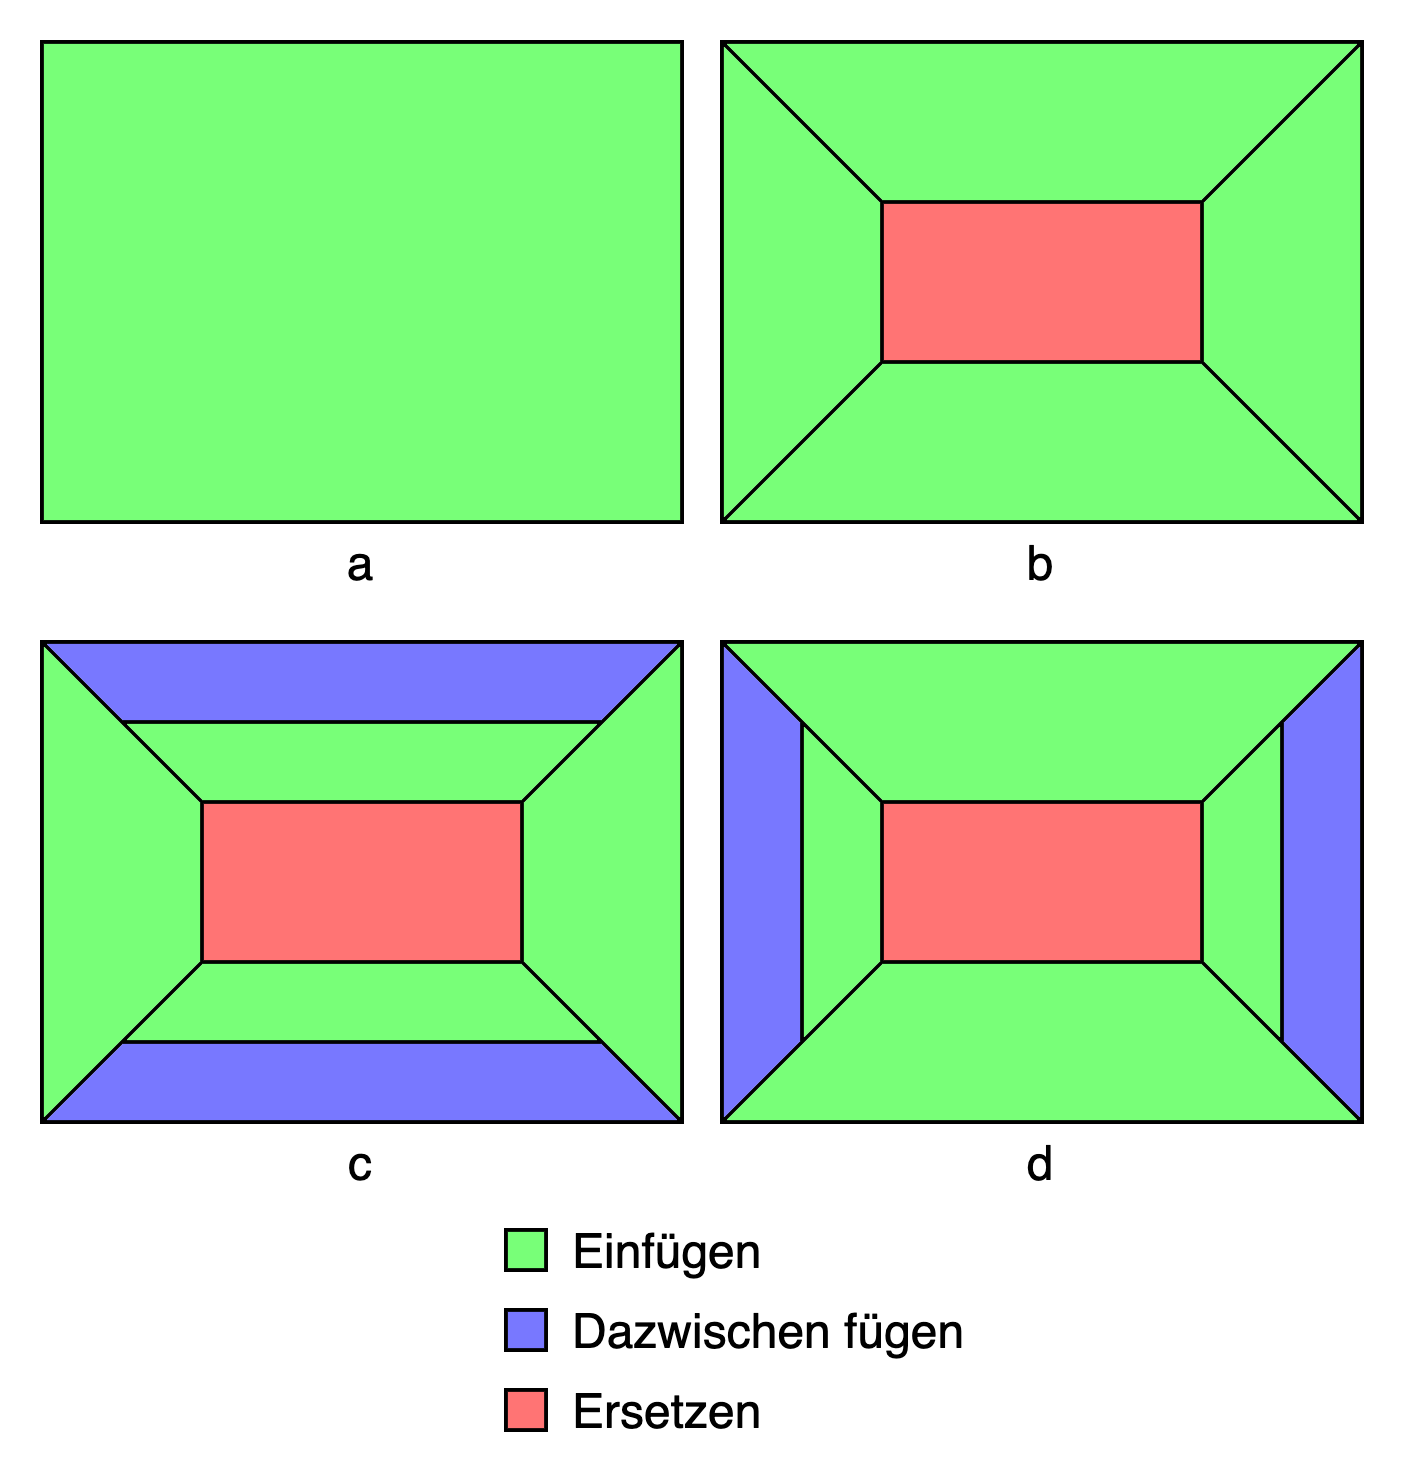
\includegraphics[scale=0.2]{img/abbildungen/DiagrammanordnungsverfahrenMitLegende}
    \end{center}
    \caption{Diagrammanordnunsverfahren}
    \label{figure:diagrammanordnungabbildung}
\end{figure}

Die Diagramme sollen nach und nach per Drag and Drop in das Dashboard integriert werden. Dieses Verfahren
wird in Abbildung \ref{figure:diagrammanordnungabbildung} dargestellt. \(a\) beschreibt den
initialen Zustand eines leeren Dashboards. Hier kann man durch Drag and Drop das erste Diagramm dem Dashboard
zuordnen. \(b\) beschreibt den Zustand des Dashboards mit genau einem enthaltenen Diagramm. Hier kann man das
neue Diagramm in alle Richtungen einfügen. Dabei Teilt das bestehende Diagram den Platz mit dem neuen gleichmäßig
auf. Bei der mittigen Positionierung wird das vorhandene Diagramm durch das neue ersetzt. \(c\) und \(d\)
beschreiben den Zustand, bei dem sich mehr als ein Diagramm im Dashboard befindet. Wenn man im Zustand \(b\)
ein Diagramm oberhalb oder unterhalb einfügt, bilden die beiden Diagramme eine Spalte. Beide dieser Diagramme
beinhalten nun den Zustand \(c\). Additional zu den möglichkeiten von Zustand \(b\), kann hier ein Diagramm
auch dazwischen gefügt werden. Es teilt sich dann den Platz mit den anderen Diagrammen in der Spalte.
Fügt man bei Zustand \(b\) ein Diagramm links oder rechts ein, bilden die beiden Diagramme eine Reihe.
Beide dieser Diagramme befinden sich nun in Zustand \(d\). Additional zu Zustand \(b\) können hier nun
auch neue Diagramme in der gleichen Reihe positioniert werden. Diese Reihen und Spalten können sich
immer weiter verschachteln. Somit kann der Benutzer mit einem ziemlich einfachen, intuitiven Verfahren
das Dashboard mit Diagrammen füllen. Durch einen Button in der Ecke rechts oben im Diagramm-Fenster
können diese auch wieder gelöscht werden. Dabei verhalten sich die zuvor beschriebenen Verfahren einfach rückläufig.
Die Anordnung der Diagramme wird als Baumstruktur im JSON-Format in der Datenbank persistiert.

\subsection{Zuweisung von Datenquellen}
\label{subsec:zuweisungungvondatenquellen}

\section{Darstellung}
\label{sec:darstellung}

\subsection{Pluginverfahren}
\label{subsec:pluginverfahren}
% Bündelung der Bibliotheken

Die Arbeit verfolgt auch für das Frontend einen Microservice-Ansatz. Man spricht hier von einem
Microfrontend. Michael Geers schreibt dazu in einem Artikel auf Digital Pioneers folgendes:
"Der Ansatz, der sich jetzt förmlich aufdrängt, ist die Umsetzung der Microservice-Idee
auch im Frontend. Anstatt einer ­großen Single-Page-Applikation baut man mehrere unabhängige
Teilapplikationen, die miteinander kommunizieren. Diese sind dann deutlich einfacher zu verstehen.
Der Einsatz einer neuen Technologie lässt sich in einem kleineren Rahmen testen."\cite{MicrofrontendT3N}
Dabei sollen die Diagramme eines Dashboards als einzelne Services ausgelagert werden.
Die Diagramme können so einzeln entwickelt und ausgeliefert werden. Aufgrund der
gleichen Machenschaft der Schnittstellen der Diagramme, kann man diese Art des Code-Splittings auch als
einen Plugin-Ansatz ansehen. Die Diagramme sollen über die In-Memory-Datenbank
Redis zur Verfügung gestellt werden. Die Diagramme werden mithilfe
von Dynamic Imports\footnote{Dynamic Imports gibt es seit ES6 (ECMAScript 2015)\cite{DynamicImportsV8}}
während der Laufzeit agil nachgeladen. Da immer nur die verwendeten Diagramme aus der In-Memory-Datenbank
geladen werden, kann die Webanwendung eine nahezu unendliche Auswahl an möglichen Diagrammen zur Visualisierung
der Daten bereitstellen.

\section{Speicherung}
\label{sec:speicherung}

\subsection{Aufbau des Dashboards}
\label{subsec:aufbaudesdashboards}

\subsection{Datenquellen und Einstellungen}
\label{subsec:datenquellenundeinstellungen}
